
%%%%%%%%%%%%%%%%%%%%%%%%%%%%%%%%%%%%%%%%%
% Journal Article
% LaTeX Template
% Version 2.0 (February 7, 2023)
%
% This template originates from:
% https://www.LaTeXTemplates.com
%
% Author:
% Vel (vel@latextemplates.com)
%
% License:
% CC BY-NC-SA 4.0 (https://creativecommons.org/licenses/by-nc-sa/4.0/)
%
% NOTE: The bibliography needs to be compiled using the biber engine.
%
%%%%%%%%%%%%%%%%%%%%%%%%%%%%%%%%%%%%%%%%%

%----------------------------------------------------------------------------------------
%	PACKAGES AND OTHER DOCUMENT CONFIGURATIONS
%----------------------------------------------------------------------------------------

\documentclass[
	a4paper, % Paper size, use either a4paper or letterpaper
	12pt, % Default font size, can also use 11pt or 12pt, although this is not recommended
	unnumberedsections, % Comment to enable section numbering
	twoside, % Two side traditional mode where headers and footers change between odd and even pages, comment this option to make them fixed
]{LTJournalArticle}

% \runninghead{Jurnal - 1313618030 - Farhan Herdian Pradana } % A shortened article title to appear in the running head, leave this command empty for no running head

% \footertext{\textit{Journal of Biological Sampling} (2024) 12:533-684} % Text to appear in the footer, leave this command empty for no footer text

%equation
\usepackage{amsmath}
\allowdisplaybreaks

%algoritma
\usepackage{algorithm}
\usepackage{algpseudocode}

\makeatletter
\newenvironment{breakablealgorithm}
{
    \begin{center}
        \refstepcounter{algorithm}
        \renewcommand{\caption}[1]
        {
            \addcontentsline{loa}{algorithm}{\protect\numberline{\thealgorithm}##1}
            \parbox{\textwidth}
            % Makes a unbreakable block and can also be done by `minipage`.
            {
                \hrule height.8pt depth0pt \kern2pt
                {\raggedright\textbf{\fname@algorithm~\thealgorithm} ##1\par}
                \kern2pt\hrule\kern2pt
            }
        }
}
{
        \kern2pt\hrule\relax
    \end{center}
}
\makeatother

\setcounter{page}{1} % The page number of the first page, set this to a higher number if the article is to be part of an issue or larger work

%----------------------------------------------------------------------------------------
%	TITLE SECTION
%----------------------------------------------------------------------------------------

\title{Perbandingan Implementasi Algoritma-algoritma Pagerank pada Satu Mesin Komputer} % Article title, use manual lines breaks (\\) to beautify the layout

% Authors are listed in a comma-separated list with superscript numbers indicating affiliations
% \thanks{} is used for any text that should be placed in a footnote on the first page, such as the corresponding author's email, journal acceptance dates, a copyright/license notice, keywords, etc
\author{%
	Farhan Herdian Pradana\textsuperscript{1}, Muhammad Eka Suryana\textsuperscript{2}, Med Irzal\textsuperscript{3}
}

% Affiliations are output in the \date{} command
\date{
	\footnotesize
	Program Studi Ilmu Komputer, Fakultas Matematika dan Ilmu Pengetahuan Alam \\
	Universitas Negeri Jakarta, DKI Jakarta, Indonesia \\
	\textsuperscript{\textbf{1}}farhan.herdia123@gmail.com, 
	\textsuperscript{\textbf{2}}eka-suryana@unj.ac.id, 
	\textsuperscript{\textbf{3}}medirzal@unj.ac.id
}

% Full-width abstract
\renewcommand{\abstractname}{Abstrak}
\renewcommand{\maketitlehookd}{%
	\begin{abstract}
		\noindent Algoritma Pagerank merupakan algoritma mengurutkan halaman web pada \textit{search engine} Google. Masalah pada Algoritma Pagerank adalah memerlukan memori utama yang cukup besar, dan tidak mungkin dilakukan pada satu mesin komputer dengan memori utama yang terbatas. Akan dicari algoritma alternatif dari Algoritma Pagerank Original buatan Google dengan membandingkannya pada algoritma-algoritma Pagerank dari penelitian lainnya dengan membandingkan kecepatan, penggunaan memori utama, dan kemiripan hasil. Penelitian dilakukan dengan melakukan pengkodean terhadap algoritma Pagerank Original, algoritma Distributed Pagerank Computation (DPC), algoritma Modified DPC (MDPC), dan algoritma Random Walker. Semua kode program dijalankan pada dataset dan dibandingkan kecepatan, penggunaan memori utama, dan kemiripan hasil akhirnya. Khusus hasil akhir, hasil dari algoritma Random Walker dijadikan acuan karena dasar dari Algoritma Pagerank adalah Random Walker. Hasilnya Algoritma Pagerank Original unggul dari sisi kecepatan dan hasil yang mirip dengan hasil Algoritma Random Walker. Sedangkan algoritma DPC dan MDPC unggul di penggunaan memori utama yang lebih hemat, sehingga cocok untuk satu mesin komputer yang memiliki memori utama yang terbatas, tetapi dengan catatan mengorbankan kecepatan yang lebih lambat dan hasil yang tidak mirip terhadap Random Walker.
	\end{abstract}
}

%----------------------------------------------------------------------------------------

\begin{document}

\maketitle % Output the title section

%----------------------------------------------------------------------------------------
%	ARTICLE CONTENTS
%----------------------------------------------------------------------------------------

\section{I. PENDAHULUAN}

Internet adalah jaringan luas yang membuat jaringan komputer seluruh dunia yang dijalankan oleh perusahaan, pemerintahan, universitas, dan organisasi lainnya untuk dapat saling berkomunikasi \citep{sample2018internet}. Internet memiliki banyak kegunaan. Di bidang komunikasi, Internet melahirkan \textit{Voice over Internet Protocol} (VoIP) dan surat elektronik (\textit{email}). Di bidang pengiriman data, internet memungkinkan pengguna untuk dapat mengunggah berkas ke \textit{file server} untuk dibagikan ke orang lain atau supaya bisa diakses di mana saja. Yang paling populer, selain dari dua bidang tersebut, internet melahirkan World Wide Web (WWW) yang memungkinkan situs web atau biasa disebut \textit{website} untuk bisa diakses oleh semua orang.

\textit{Website} adalah sekumpulan halaman web yang saling terkait dan berada pada nama domain yang sama. Website dapat dibuat dan dipelihara oleh seorang individu, grup, perusahaan, atau organisasi lain dengan berbagai macam tujuan \citep{techopedia2020website}. Dengan adanya \textit{website}, kegunaan internet menjadi semakin lebih luas, lebih berkualitas, dan lebih mudah digunakan. \textit{Website} yang menggunakan protokol HTTP, memungkinkan untuk mengirim berkas HTML, CSS, dan JavaScript sehingga internet dapat menampilkan visual yang lebih ramah terhadap pengguna dan menjadi media hiburan baru. Tidak heran, \textit{website} terus tumbuh pesat. Pada tahun 1992 hanya terdapat sepuluh \textit{website}, lalu pada tahun 1994 angka ini bertumbuh menjadi 3.000 \textit{website}, dan semakin bertumbuh pesat pada tahun 2021 menjadi kurang lebih 1,88 miliar \textit{website} \citep{amstrong2021website}.

Dengan meledaknya jumlah halaman web, memunculkan tantangan baru dalam memperoleh informasi dari web. Pengguna biasanya menelusuri web dengan mengunjungi graf \textit{link} yang terdapat pada halaman web, biasanya dimulai pada situs kumpulan index halaman web berkualitas tinggi yang dipelihara oleh manusia seperti Yahoo.com, atau menggunakan \textit{search engine} \citep{brin1998anatomy}. Seiring perkembangan zaman, \textit{search engine} Google menjadi \textit{search engine} teratas dengan pengguna terbesar di dunia dengan penguasaan pasar sebesar 91\% \citep{gsc2022marketshare}. Google awalnya merupakan proyek Sergey Brin dan Larry Page saat mereka mengambil gelar Ph.D di Universitas Stanford dengan tujuan membuat \textit{search engine} yang lebih berkualitas dibandingkan \textit{search engine} lain \citep{brin1998anatomy}. Kunci kesuksesan dari Google terletak pada Pagerank. Pagerank merangking halaman web berdasarkan kepentingan relatif (\textit{relative importance}) suatu halaman web berdasarkan graf tautan web \citep{ilprints422}. Sebelum adanya Pagerank, \textit{search engine} lain biasanya merangking suatu halaman web dengan menghitung banyaknya \textit{backlink} yang merujuk halaman tersebut \citep{ilprints422}. Metode tersebut akan menjadi mudah untuk dimanipulasi pemilik halaman web yang ingin mendapatkan \textit{ranking} teratas dengan membuat halaman web lain yang berisi \textit{link} yang menunjuk pada halaman web tujuan sebanyak-banyaknya. Pagerank menjawab permasalahan tersebut dengan melakukan normalisasi pada jumlah \textit{backlink} suatu halaman web \citep{brin1998anatomy}. Hal ini yang membuat hasil pencarian Google menjadi lebih relevan dibandingkan hasil pencarian \textit{search engine} lain.

Setiap \textit{search engine} memiliki arsitektur berbeda-beda. Arsitektur Google dipilih dan dijadikan acuan dalam topik penelitian peningkatan arsitektur \textit{search engine} yang merupakan penelitian induk dari judul penelitian ini karena keunggulannya dibandingkan \textit{search engine} lain. Arsitektur Google dapat dilihat pada gambar \ref{gambar:google_architecture_filled}. Modul \textit{crawler} dan pendukungnya yang ditandai dengan warna biru muda sudah dibuat pada penelitian sebelumnya yang berjudul "Perancangan \textit{Crawler} Sebagai Pendukung Pada Search Engine" oleh \citet{qoriiba2021perancangan}. Pada penelitian tersebut digunakan algoritma \textit{modified similarity based crawling} dan selanjutnya hasil dari \textit{crawling} disimpan kedalam \textit{database} MySQL \citep{qoriiba2021perancangan}. Selanjutnya penelitian berjudul "Perancangan Arsitektur \textit{Search Engine} dengan Mengintegrasikan \textit{Web Crawler}, Algoritma Page \textit{ranking}, dan Dokumen \textit{ranking}" oleh \citet{khatulistiwa2022SearchEngine}. Pada penelitian tersebut digabungkan modul \textit{crawler} dari penelitian \citet{qoriiba2021perancangan}, Pagerank, dan \textit{searcher} pada penelitian lain sebelumnya menjadi \textit{search engine} berbasis konsol \citep{khatulistiwa2022SearchEngine}. Pada modul \textit{indexer} dilakukan penelitian oleh \citet{pratama2022indexer} berjudul "Perancangan Modul Pengindeks pada \textit{Search Engine} Berupa \textit{Induced Generalized Suffix Tree} untuk Keperluan Perangkingan Dokumen" dan \citet{zalghornain2022indexer} berjudul "Rancang Bangun Sistem Pencarian Teks dengan Menggunakan Model \textit{Continuous-Bag-of-Words} dan Model \textit{Continuous Skip-Gram} pada Koleksi Dokumen".

Dalam melakukan perangkingan halaman web, Pagerank dapat didefinisikan pada persamaan \ref{eq:1}. Dimana $u$ adalah halaman web. $F_u$ adalah himpunan halaman $u$ yang menunjuk halaman lain dan $B_u$ adalah himpunan halaman yang menunjuk ke $u$. $C_u = |F_u|$ adalah jumlah \textit{link} dari $u$ dan $c$ adalah faktor yang digunakan untuk normalisasi (sehingga jumlah total \textit{ranking} semua halaman web adalah konstan) dan $c < 1$. $E(u)$ adalah vektor yang berkorespondensi dengan \textit{ranking} halaman web. $||\pi'||_1 = 1$. Iterasi perhitungan terus dilakukan sampai konvergen. Jika diubah kedalam persamaan matriks, maka persamaan \ref{eq:1} dapat diubah menjadi persamaan \ref{eq:2}. Dimana $X$ adalah matriks persegi yang baris dan kolomnya berkorespondensi dengan halaman web, dengan elemen $X_{u,v} = \frac{1}{C_u}$ jika terdapat \textit{link} pada halaman $u$ ke halaman $v$ atau $X_{u,v} = 0$ jika tidak ada.

\begin{equation}
	\label{eq:1}
	\pi'(u) = c\sum_{v\in B_u} \frac{\pi'(v)}{C_v} + cE(u)
\end{equation}

\begin{equation}
	\label{eq:2}
	\pi'=c(X\pi' + E)
\end{equation}

Dasar intuitif dari persamaan \ref{eq:1} adalah \textit{random walks} pada sebuah graf. Anggap pengguna internet sebagai \textit{"random surfer"} yang terus meng-klik \textit{link} selanjutnya secara acak. Namun, jika pengguna terjebak pada sebuah lingkaran halaman web (\textit{link} yang diklik terus menampilkan halaman web yang pernah dikunjungi sebelumnya), tidak mungkin pengguna akan terus mengikuti \textit{link} tersebut, melainkan pengguna akan langsung pindah ke halaman lain. Oleh sebab itu faktor $E$ dipakai untuk memodelkan perilaku ini (Pengguna akan bosan dan langsung lompat ke halaman web lain berdasarkan distribusi pada $E$) \citep{ilprints422}. $E$ dapat didefinisikan oleh pengguna (\textit{user-defined parameter}) dan nilai elemennya dapat diisi dengan nilai yang seragam atau berbeda-beda. Menariknya, jika nilai elemen $E$ dibuat berbeda-beda, maka dapat membuat Pagerank yang dipersonalisasi \citep{ilprints422}.

Walaupun persamaan Pagerank terlihat sederhana, terdapat masalah dari sisi ruang dan waktu. Dari sisi ruang, misal terdapat 1000 halaman web, maka akan terbentuk 1000x1000 matriks $X$. Misal tiap sel elemen $X$ memerlukan memori 8 \textit{Byte}, maka untuk membentuk 1000x1000 matriks $X$, tanpa menghitung alokasi \textit{overhead} memori, memerlukan 8 \textit{Mega Byte} (MB) memori utama (Lihat tabel \ref{table:1}). Di internet terdapat miliaran \textit{website} dan setiap \textit{website} dapat memiliki lebih dari 1 halaman, sehingga untuk bisa membentuk matriks $X$ membutuhkan memori utama dengan kapasitas mencapai \textit{Peta Byte} atau bahkan \textit{Exa Byte}. Hal tersebut sangat tidak mungkin dilakukan pada komputer pribadi biasa yang memori utamanya hanya pada kisaran 4 GB sampai 32 GB, yang berarti ketika program dieksekusi langsung \textit{crash} karena memori yang tidak cukup. Dari sisi waktu, proses \textit{string matching} untuk mengakses nilai \textit{ranking} suatu halaman web berdasarkan \textit{string} URLnya juga memiliki kompleksitas waktu yang besar yakni O(NM), jika dilakukan dengan cara dicari satu-persatu. Beruntung \textit{database} seperti MySQL menggunakan B-Tree dalam mengindeks datanya \citep{mysqlIndex}. B-tree memiliki kompleksitas waktu kecil yakni hanya O(log(n)) \citep{geeksForGeeksBtree}.


\begin{table}
	\centering
	\caption{Tabel alokasi memori utama untuk membentuk matriks $X$}
	\label{table:1}
	\begin{tabular}{|c|c|} 
		\hline
		Jumlah Halaman Web & Memori (\textit{Byte}) \\
		\hline
		
		\hline
		256 & 524416 \\
		512 & 2097280 \\
		1024 & 8388736 \\
		2048 & 33554560 \\
		4096 & 134217856 \\
		8192 & 536871040 \\
		16384 & 2147483776 \\
		32768 & 8589934720 \\
		\hline
	\end{tabular}
\end{table}

Telah dilakukan penelitian tentang Pagerank yang terdistribusi dengan metode \textit{iterative aggregation-disaggregation} (IAD) dengan \textit{Block Jacobi smoothing} \citep{zhuetal2005distributedPagerank}. Sederhananya, dilakukan \textit{divide-and-conquer} dengan mengelompokan halaman web berdasarkan \textit{domain}-nya lalu dihitung Pagerank lokalnya dan disatukan dengan metode komunikasi yang hemat memori dengan sebuah koordinator \citep{zhuetal2005distributedPagerank}. Hasilnya, ditemukan sebuah metode Pagerank terdistribusi yang bisa dijalankan pada memori utama kecil dan lebih cepat konvergen sehingga menghemat waktu \citep{zhuetal2005distributedPagerank}. Oleh karena itu, akan dicari algoritma Pagerank alternatif yang dapat dijalankan pada satu mesin komputer dengan memori utama terbatas, dengan cara melakukan perbandingan implementasi beberapa algoritma Pagerank pada satu mesin komputer.

%------------------------------------------------

\section{II. Kajian Teori}

\subsection{World Wide Web (WWW)}

WWW merupakan proyek Tim Berner-lee bersama teman-temannya, yang ditunjukan pada publik pada tahun 1991. WWW didesain untuk membawa sebuah semesta informasi global menggunakan teknologi yang ada. Dengan adanya WWW manusia dapat mengakses seluruh informasi melalui sebuah \textit{platform browsing} apapun. Pada masa itu, sudah ada teknologi serupa yang membuat WWW mungkin untuk dilakukan. Sistem \textit{hypertext} yang sudah ada pada saat itu, terbatas pada sistem \textit{file} lokal atau terdistribusi dan kadang hanya dikembangkan pada \textit{platform} tertentu. Selain itu, juga ada sistem pengambilan dan akses informasi seperti Alex, Gopher, Prospero, dan WAIS yang sudah mencakup area yang luas, tetapi tanpa fungsionalitas \textit{hypertext}. WWW menggabungkan teknik \textit{hypertext}, \textit{information retrieval}, dan \textit{wide area networking} \citep{bernersLee1992}.

\begin{figure}
	\centering
	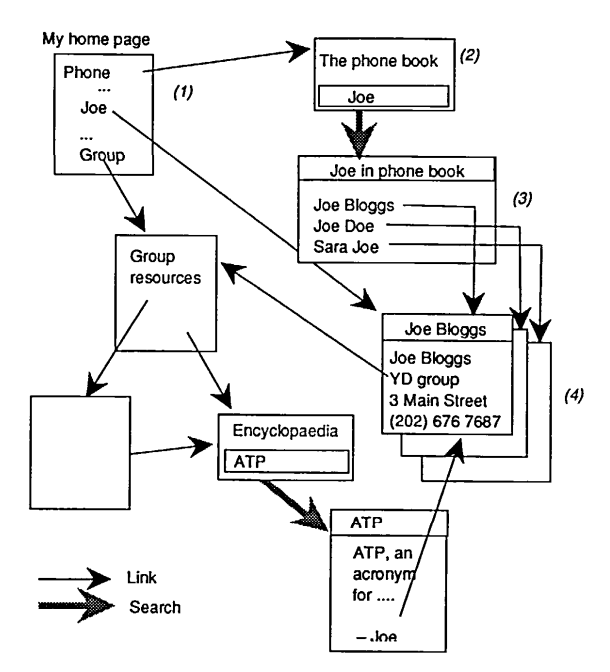
\includegraphics[width=\linewidth]{gambar/w3_model}
	\caption{Gambar sebuah web yang terdiri atas kumpulan \textit{link} dan indeks \citep{bernersLee1992}}
	\label{gambar:w3_model}
\end{figure}

Model yang dipakai WWW menggunakan dua paradigma dari \textit{hypertext link} dan pencarian teks yang saling melengkapi. Gambar \ref{gambar:w3_model} menunjukkan bagaimana sebuah web yang berisi informasi pribadi terbentuk pada paradigma ini. Pembaca mulai pada halaman \textit{home} (1) lalu menggunakan \textit{link} grup atau publik untuk mencari bahan informasi. Indeks seperti buku telepon (2) ditampilkan sebagai dokumen yang memungkinkan untuk melakukan input pencarian. Hasil dari pencarian berupa dokumen \textit{hypertext} virtual (3) yang menunjuk pada dokumen yang ditemukan (4) \citep{bernersLee1992}.

\subsection{Teori Graf}

\begin{figure}[!htb]
\begin{minipage}{0.48\textwidth}
	\centering
	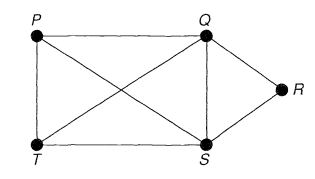
\includegraphics[width=.7\linewidth]{gambar/graph_example}
	\caption{Contoh graf \citep{wilson1996}}
	\label{gambar:graph_example}
\end{minipage}\hfill
\begin{minipage}{0.48\textwidth}
	\centering
	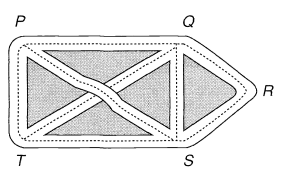
\includegraphics[width=.7\linewidth]{gambar/graph_example_2}
	\caption{Contoh peta jalan yang dapat diandaikan sebagai graf \citep{wilson1996}}
	\label{gambar:graph_example_2}
\end{minipage}
\end{figure}

\begin{figure}
	\centering
	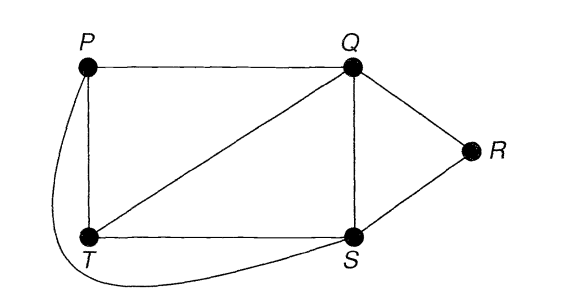
\includegraphics[keepaspectratio, width=0.48\textwidth]{gambar/graph_example_3}
	\caption{}
	\label{gambar:graph_example_3}
\end{figure}

Graf adalah sebuah representasi dari himpunan titik (\textit{node / vertice}) dan bagaimana titik-titik tersebut saling terhubung tanpa memperdulikan sifat metriknya \citep{wilson1996}. Pada gambar \ref{gambar:graph_example} merupakan contoh graf, dengan $P$, $Q$, $R$, $S$, $T$ merupakan titik, dan masing-masing terhubung dengan garis (\textit{edge}). Garis yang menghubungkan titik $P$ dan $S$ disebut dengan $PS$, sedangkan garis yang menghubungkan titik $Q$ dan $T$ disebut dengan $QT$. Persilangan antara $PS$ dan $QT$ tidak disebut sebagai titik, karena keduanya tidak saling bersilangan, melainkan saling melompati layaknya gambar \ref{gambar:graph_example_2}. Selanjutnya, kedua graf dianggap sama, jika dan hanya jika titik yang berkorespondensi sama-sama terhubung dengan garis yang sama dengan garis pada graf lainnya \citep{wilson1996}. Sebagai contoh, graf pada gambar \ref{gambar:graph_example_3} merupakan graf yang sama dengan graf pada gambar \ref{gambar:graph_example} \citep{wilson1996}. 

\begin{figure}[!htb]
\begin{minipage}{0.48\textwidth}
	\centering
	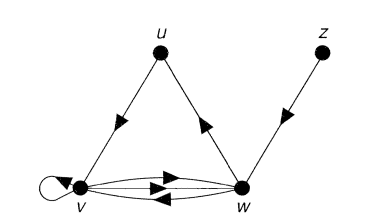
\includegraphics[width=.7\linewidth]{gambar/digraph_example}
	\caption{Contoh digraf \citep{wilson1996}}
	\label{gambar:digraph_example}
\end{minipage}\hfill
\begin{minipage}{0.48\textwidth}
	\centering
	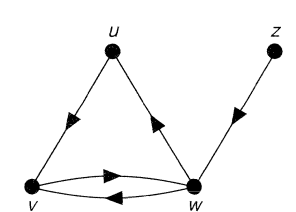
\includegraphics[width=.7\linewidth]{gambar/simple_digraph_example}
	\caption{Contoh digraf sederhana \citep{wilson1996}}
	\label{gambar:simple_digraph_example}
\end{minipage}
\end{figure}

Garis pada graf dapat diberikan arah. Garis pada graf yang berarah disebut sebagai busur (\textit{arc}). Graf yang memiliki arah pada garisnya disebut dengan graf berarah (\textit{directed graph / digraph} / digraf) yang terdiri atas himpunan titik dan busur \citep{wilson1996}. Pada digraf di gambar \ref{gambar:digraph_example} terdapat himpunan titik $u$, $v$, $w$, dan $z$, dengan busur $uv$, $vv$, $vw (2\times)$, $wv$, $wu$, dan $zw$. Sebuah digraf disebut sebagai digraf sederhana jika himpunan busurnya tidak ada yang sama (\textit{distinct}) dan tidak memiliki \textit{loop} (contoh: busur $vv$) \citep{wilson1996}. Digraf pada gambar \ref{gambar:simple_digraph_example} adalah contoh digraf sederhana.

\subsection{Pagerank}

Jika World Wide Web diibaratkan pada sebuah graf berarah, halaman web adalah titik graf, \textit{link} adalah garis. Lalu \textit{link} yang menunjuk keluar dari titik disebut \textit{forward link}, sedangkan \textit{link} yang menunjuk kedalam titik disebut \textit{backlink}. Sangat sulit untuk mengetahui semua \textit{backlink} suatu halaman web, tetapi sangat mudah untuk mengetahui semua \textit{forward link} suatu halaman web yaitu dengan cara mengunduh halaman web tersebut \citep{ilprints422}. Setiap halaman web memiliki jumlah \textit{backlink} yang beragam. Pada saat Pagerank diteliti, halaman \textit{home} NetScape memiliki 62.804 \textit{backlink} dibandingkan halaman web kebanyakan yang hanya memiliki beberapa \textit{backlink}. Secara umum suatu halaman web jika memiliki banyak \textit{backlink} dapat dianggap lebih penting daripada halaman web lain yang memiliki lebih sedikit \textit{backlink}. Perhitungan jumlah sitasi sederhana pernah digunakan untuk memprediksi pemenang Nobel masa depan \citep{ilprints422}. 

\begin{equation}
	\label{eq:5-1}
	P_{ij}= 
	\begin{cases}
		\frac{d}{C_j} + \frac{(1-d)}{N} & j \to i \\
		\frac{(1-d)}{N} & j \not\to i \text{ dan } C_j \not=0 \\
		\frac{1}{N} & C_j = 0
	\end{cases}
\end{equation}

Graf pada WWW, dapat direpresentasikan sebagai matriks transisi $P$. Matriks $P$ didefinisikan pada persamaan \ref{eq:5-1}. $C_j$ adalah jumlah \textit{forward link} dari halaman $j$. $j \to i$ adalah halaman $j$ memiliki \textit{link} menuju halaman $i$.

Selanjutnya algoritma Pagerank didefinisikan pada algoritma \ref{alg:1.1}

\begin{algorithm}
	\floatname{algorithm}{Algoritma}
	\caption{Pagerank \citep{zhuetal2005distributedPagerank}}
	\label{alg:1.1}
	\begin{algorithmic}[1]
		\State Definisikan $\pi^0$ awal-awal
		\State $k \gets 0$
		\State \label{alg:1.1.step:start_loop} $\pi^{\sim k+1} \gets P \pi^k$
		\State $\pi^{k+1} \gets \frac{\pi^{\sim k+1}}{||\pi^{\sim k+1}||_1}$
		\State Jika $||\pi^{k+1} - \pi^k|| < \epsilon$  berhenti dan kembalikan nilai $\pi^{k+1}$
		\State $k \gets k+1$
		\State Ulangi langkah \ref{alg:1.1.step:start_loop}
	\end{algorithmic}
\end{algorithm}

\subsection{Distributed Pagerank Computation (DPC)}

Telah dijelaskan sebelumnya, masalah dari algoritma Pagerank biasa adalah besarnya memori utama yang dibutuhkan untuk bisa menyimpan matriks $X$ (lihat persamaan \ref{eq:2}). Oleh karena itu, dirumuskan algoritma Pagerank terdistribusi. DPC, dirumuskan oleh \citet{zhuetal2005distributedPagerank}, memakai mekanisme interaksi sederhana antara \textit{cluster} dan lalu lintas komunikasi rendah. Ditinjau dari perspektif matematika, dibuktikan bahwa algoritma DPC setara dengan metode \textit{Iterative Aggregation-Disaggregation} (IAD) dengan \textit{Block Jacobi smoothing}. DPC juga memiliki keunggulan dibandingkan dengan algoritma Pagerank biasa yaitu, matriks-matriks dipecah menjadi matriks agregasi dan matriks lokal sehingga ukurannya cukup kecil untuk disimpan di memori utama, sehingga mempercepat komputasi karena tiap iterasi memerlukan sedikit operasi I/O pada \textit{disk}. Selanjutnya, Vektor Pagerank lokal konvergen lebih cepat pada beberapa \textit{cluster} tertentu, berbeda dengan Pagerank biasa karena terdapat komputasi tidak perlu pada \textit{cluster} yang sudah konvergen \citep{zhuetal2005distributedPagerank}.

Jika \textit{link} pada kumpulan web dibuat kedalam graf, maka graf tersebut akan memiliki sebuah struktur menyerupai blok, karena mayoritas dari \textit{link} tersebut bersifat \textit{intra-host}, merujuk halaman yang masih di dalam \textit{host} yang sama. Oleh karena itu, jika dilakukan perjalanan acak pada kumpulan web tersebut dapat dilihat sebagai rantai Markov \textit{Nearly Completely Decomposable} (NCD) \citep{zhuetal2005distributedPagerank}. Rantai Markov NCD adalah rantai Markov yang dapat dipartisi sehingga peluang dari keadaan awal ke keadaan selanjutnya lebih sering menunjuk keadaan yang berada di dalam partisinya dibandingkan di luar partisinya \citep{kontovasilisMitrou1995}.

Sebelum langsung membahas algoritma DPC, akan didefinisikan beberapa notasi terlebih dahulu. $e=(1,...,1)^T$. Misal G adalah himpunan bilangan bulat $\{1,...,N\}$. Misal $G_1,...G_n, n \leq N$ adalah grup agregasi dari elemen-elemen di $G$. Himpunan-himpunan $G_i, i = 1,...,n$, adalah saling lepas dan $\cup^n_{i=1}G_i=G$. Misal $N_i$ adalah ordo dari himpunan $G_i$, atau jumlah elemen-elemen di $G_i$ \citep{zhuetal2005distributedPagerank}. 

Misal $R$ adalah matriks agregasi $n \times N$, yang memenuhi persamaan \ref{eq:3} \citep{zhuetal2005distributedPagerank}.

\begin{equation}
	\label{eq:3}
	R_{ij}= 
	\begin{cases}
			1 & j \in G_i\\
			0 & \text{lainnya}
	\end{cases}
\end{equation}

Dilakukan partisi pada vektor positif $\pi$ menjadi $(\pi^T_1,\pi^T_2,...,\pi^T_n)^T$ berdasarkan $\{G_i\}$. $\pi_i$ adalah subvektor dengan dimensi $N_i$ \citep{zhuetal2005distributedPagerank}.

Maka dapat didefinisikan matriks disagregasi $S(\pi)$ $N \times n$ sebagai persamaan \ref{eq:4} \citep{zhuetal2005distributedPagerank}.
\begin{equation}
	\label{eq:4}
	S(\pi) = 
	\begin{pmatrix}
		S(\pi)_1 & 0 & \ldots & 0 \\
		0 & S(\pi)_2 & \ldots & 0 \\
		\vdots & \vdots & \ddots & \vdots \\
		0 & 0 & \ldots & S(\pi)_n
	\end{pmatrix}
\end{equation}
Dimana $S(\pi)_i$ adalah sebuah kolom vektor yang mewakili \textit{censored stationary distribution} dari halaman-halaman di \textit{cluster} $G_i$. Ingat bahwa $RS(\pi) = I$ \citep{zhuetal2005distributedPagerank}.

Matriks transisi $P$ dipartisi menjadi beberapa blok berdasarkan $\{G_i\}$ menjadi seperti persamaan \ref{eq:6} \citep{zhuetal2005distributedPagerank}.
\begin{equation}
\label{eq:6}
	P =
	\begin{pmatrix}
		P_{11} & P_{12} & \ldots & P_{1n} \\
		P_{21} & P_{22} & \ldots & P_{2n} \\
		\vdots & \vdots & \ddots & \vdots \\
		P_{n1} & P_{n2} & \ldots & P_{nn}
	\end{pmatrix}
\end{equation}
Dilambangkan blok baris ke-$i$ sebagai persamaan \ref{eq:7}
\begin{equation}
\label{eq:7}
	P_{i*} \overset{\Delta}{=} (P_{i1},\ldots,P_{in})
\end{equation}
dan dilambangkan blok kolom ke-$i$ sebagai persamaan \ref{eq:8}
\begin{equation}
\label{eq:8}
	P_{*i} \overset{\Delta}{=}
	\begin{pmatrix}
		P_{1i} \\
		\vdots \\
		P_{ni} 
	\end{pmatrix}
\end{equation} 

Setiap blok diagonal $P_{ii}$ adalah matriks persegi dan merupakan matriks \textit{intra-cluster} \textit{link} dari \textit{cluster} $G_i$, sementara blok-blok di luar diagonal merupakan struktur \textit{link} antar-\textit{cluster}. Selanjutnya, matriks agregat $A = RPS(\pi)$ adalah matriks transisi antar \textit{cluster}. Maka dapat dibuat algoritma DPC pada algoritma \ref{alg:3} \citep{zhuetal2005distributedPagerank}.

\begin{breakablealgorithm}
\label{alg:3}
\floatname{algorithm}{Algoritma}
\caption{Algoritma DPC \citep{zhuetal2005distributedPagerank}}
\begin{algorithmic}[1]
  \State Buat matriks transisi lokal untuk tiap \textit{cluster} $G_i$ berdasarkan $P$ 
		\begin{equation} \label{alg:3.step:trivial:1} Q_i = LocalTransitionMatrix(G_i) \forall G_i \in G \end{equation}
  \State 
		\begin{equation} \label{alg:3.step:trivial:2} \pi_i^0 = Pagerank(Q_i, \frac{e}{N_i}, \epsilon) \forall G_i \in G \end{equation}
		Ket: $e = [1, 1, ..., 1]^T; N_i \rightarrow \text{jumlah anggota $G_i$}$
  \State Inisialisasi $k = 0$
	\State
		\begin{equation} \label{alg:3.step:2:1} A^k = RPS(\pi^k) \end{equation}
		Ket: $R \rightarrow \text{persamaan \ref{eq:3}}; P \rightarrow \text{persamaan \ref{eq:5-1}}; S(\pi) \rightarrow \text{persamaan \ref{eq:4}}$
	\State
		\begin{equation} \label{alg:3.step:2:2} z^k = Pagerank(A^k, \frac{e}{n}, \epsilon) \end{equation}
		Ket: $n \rightarrow \text{banyaknya anggota }G$
	\State \label{alg:3.step:3:1} $\forall G_i \in G$ buat sebuah \textit{extended local transition matrix} $(N_i + 1) \times (N_i + 1)$. Dimana skalar $\alpha^k$ membuat jumlah nilai kolom dari $B^k_i$ adalah satu
		\begin{equation}
			\label{eq:9}
			B_i^k =
			\begin{pmatrix}
				P_{ii} 		& \frac{(P_{i*}S(\pi^k)z^k - P_{ii}\pi_i^kz_i)}{(1 - z^k_i)} \\
				e^TP_{*i} & \alpha^k
			\end{pmatrix}
		\end{equation}
	\State \label{alg:3.step:3:2} Hitung vektor \textit{extended local Pagerank}. Dimana $\beta^{k+1}_i$ adalah skalar
		\begin{equation}
			\begin{pmatrix}
				\omega^{k+1}_i \\
				\beta^{k+1}_i
			\end{pmatrix}
			= Pagerank(B^k_i, \frac{e}{(N_i + 1)}, \epsilon)
		\end{equation}
	\State \label{alg:3.step:3:3} \begin{equation} \pi^{\sim k+1}_i = \frac{1 - z^k_i}{\beta^{k+1}_i} \omega^{k+1}_i \end{equation}
	\State \label{alg:3.step:normalization} \begin{equation} \pi^{k+1} = \frac{\pi^{\sim k+1}}{||\pi^{\sim k+1}||_1} \end{equation}
	\State $k = k+1$
	\State Jika persamaan \ref{alg:3.eq:1} terpenuhi, berhenti dan berikan $\pi^{k}$ sebagai hasil akhir. Jika sebaliknya, kembali ke langkah \ref{alg:3.step:2:1}
		\begin{equation} \label{alg:3.eq:1} ||\pi^{k+1} - \pi^k|| < \epsilon \end{equation}
\end{algorithmic}
\end{breakablealgorithm}

%------------------------------------------------

\section{Results}

\begin{table} % Single column table
	\caption{Example single column table.}
	\centering
	\begin{tabular}{l l r}
		\toprule
		\multicolumn{2}{c}{Location} \\
		\cmidrule(r){1-2}
		East Distance & West Distance & Count \\
		\midrule
		100km & 200km & 422 \\
		350km & 1000km & 1833 \\
		600km & 1200km & 890 \\
		\bottomrule
	\end{tabular}
	\label{tab:distcounts}
\end{table}

Referencing a table using its label: Table \ref{tab:distcounts}.

\begin{table*} % Full width table (notice the starred environment)
	\caption{Example two column table with fixed-width columns.}
	\centering % Horizontally center the table
	\begin{tabular}{L{0.2\linewidth} L{0.2\linewidth} R{0.15\linewidth}} % Manually specify column alignments with L{}, R{} or C{} and widths as a fixed amount, usually as a proportion of \linewidth
		\toprule
		\multicolumn{2}{c}{Location} \\
		\cmidrule(r){1-2}
		East Distance & West Distance & Count \\
		\midrule
		100km & 200km & 422 \\
		350km & 1000km & 1833 \\
		600km & 1200km & 890 \\
		\bottomrule
	\end{tabular}
\end{table*}

Aenean feugiat pellentesque venenatis. Sed faucibus tristique tortor vel ultrices. Donec consequat tellus sapien. Nam bibendum urna mauris, eget sagittis justo gravida vel. Mauris nisi lacus, malesuada sit amet neque ut, venenatis tempor orci. Curabitur feugiat sagittis molestie. Duis euismod arcu vitae quam scelerisque facilisis. Praesent volutpat eleifend tortor, in malesuada dui egestas id. Donec finibus ac risus sed pellentesque. Donec malesuada non magna nec feugiat. Mauris eget nibh nec orci congue porttitor vitae eu erat. Sed commodo ipsum ipsum, in elementum neque gravida euismod. Cras mi lacus, pulvinar ut sapien ut, rutrum sagittis dui. Donec non est a metus varius finibus. Pellentesque rutrum pellentesque ligula, vitae accumsan nulla hendrerit ut.

\begin{figure} % Single column figure
	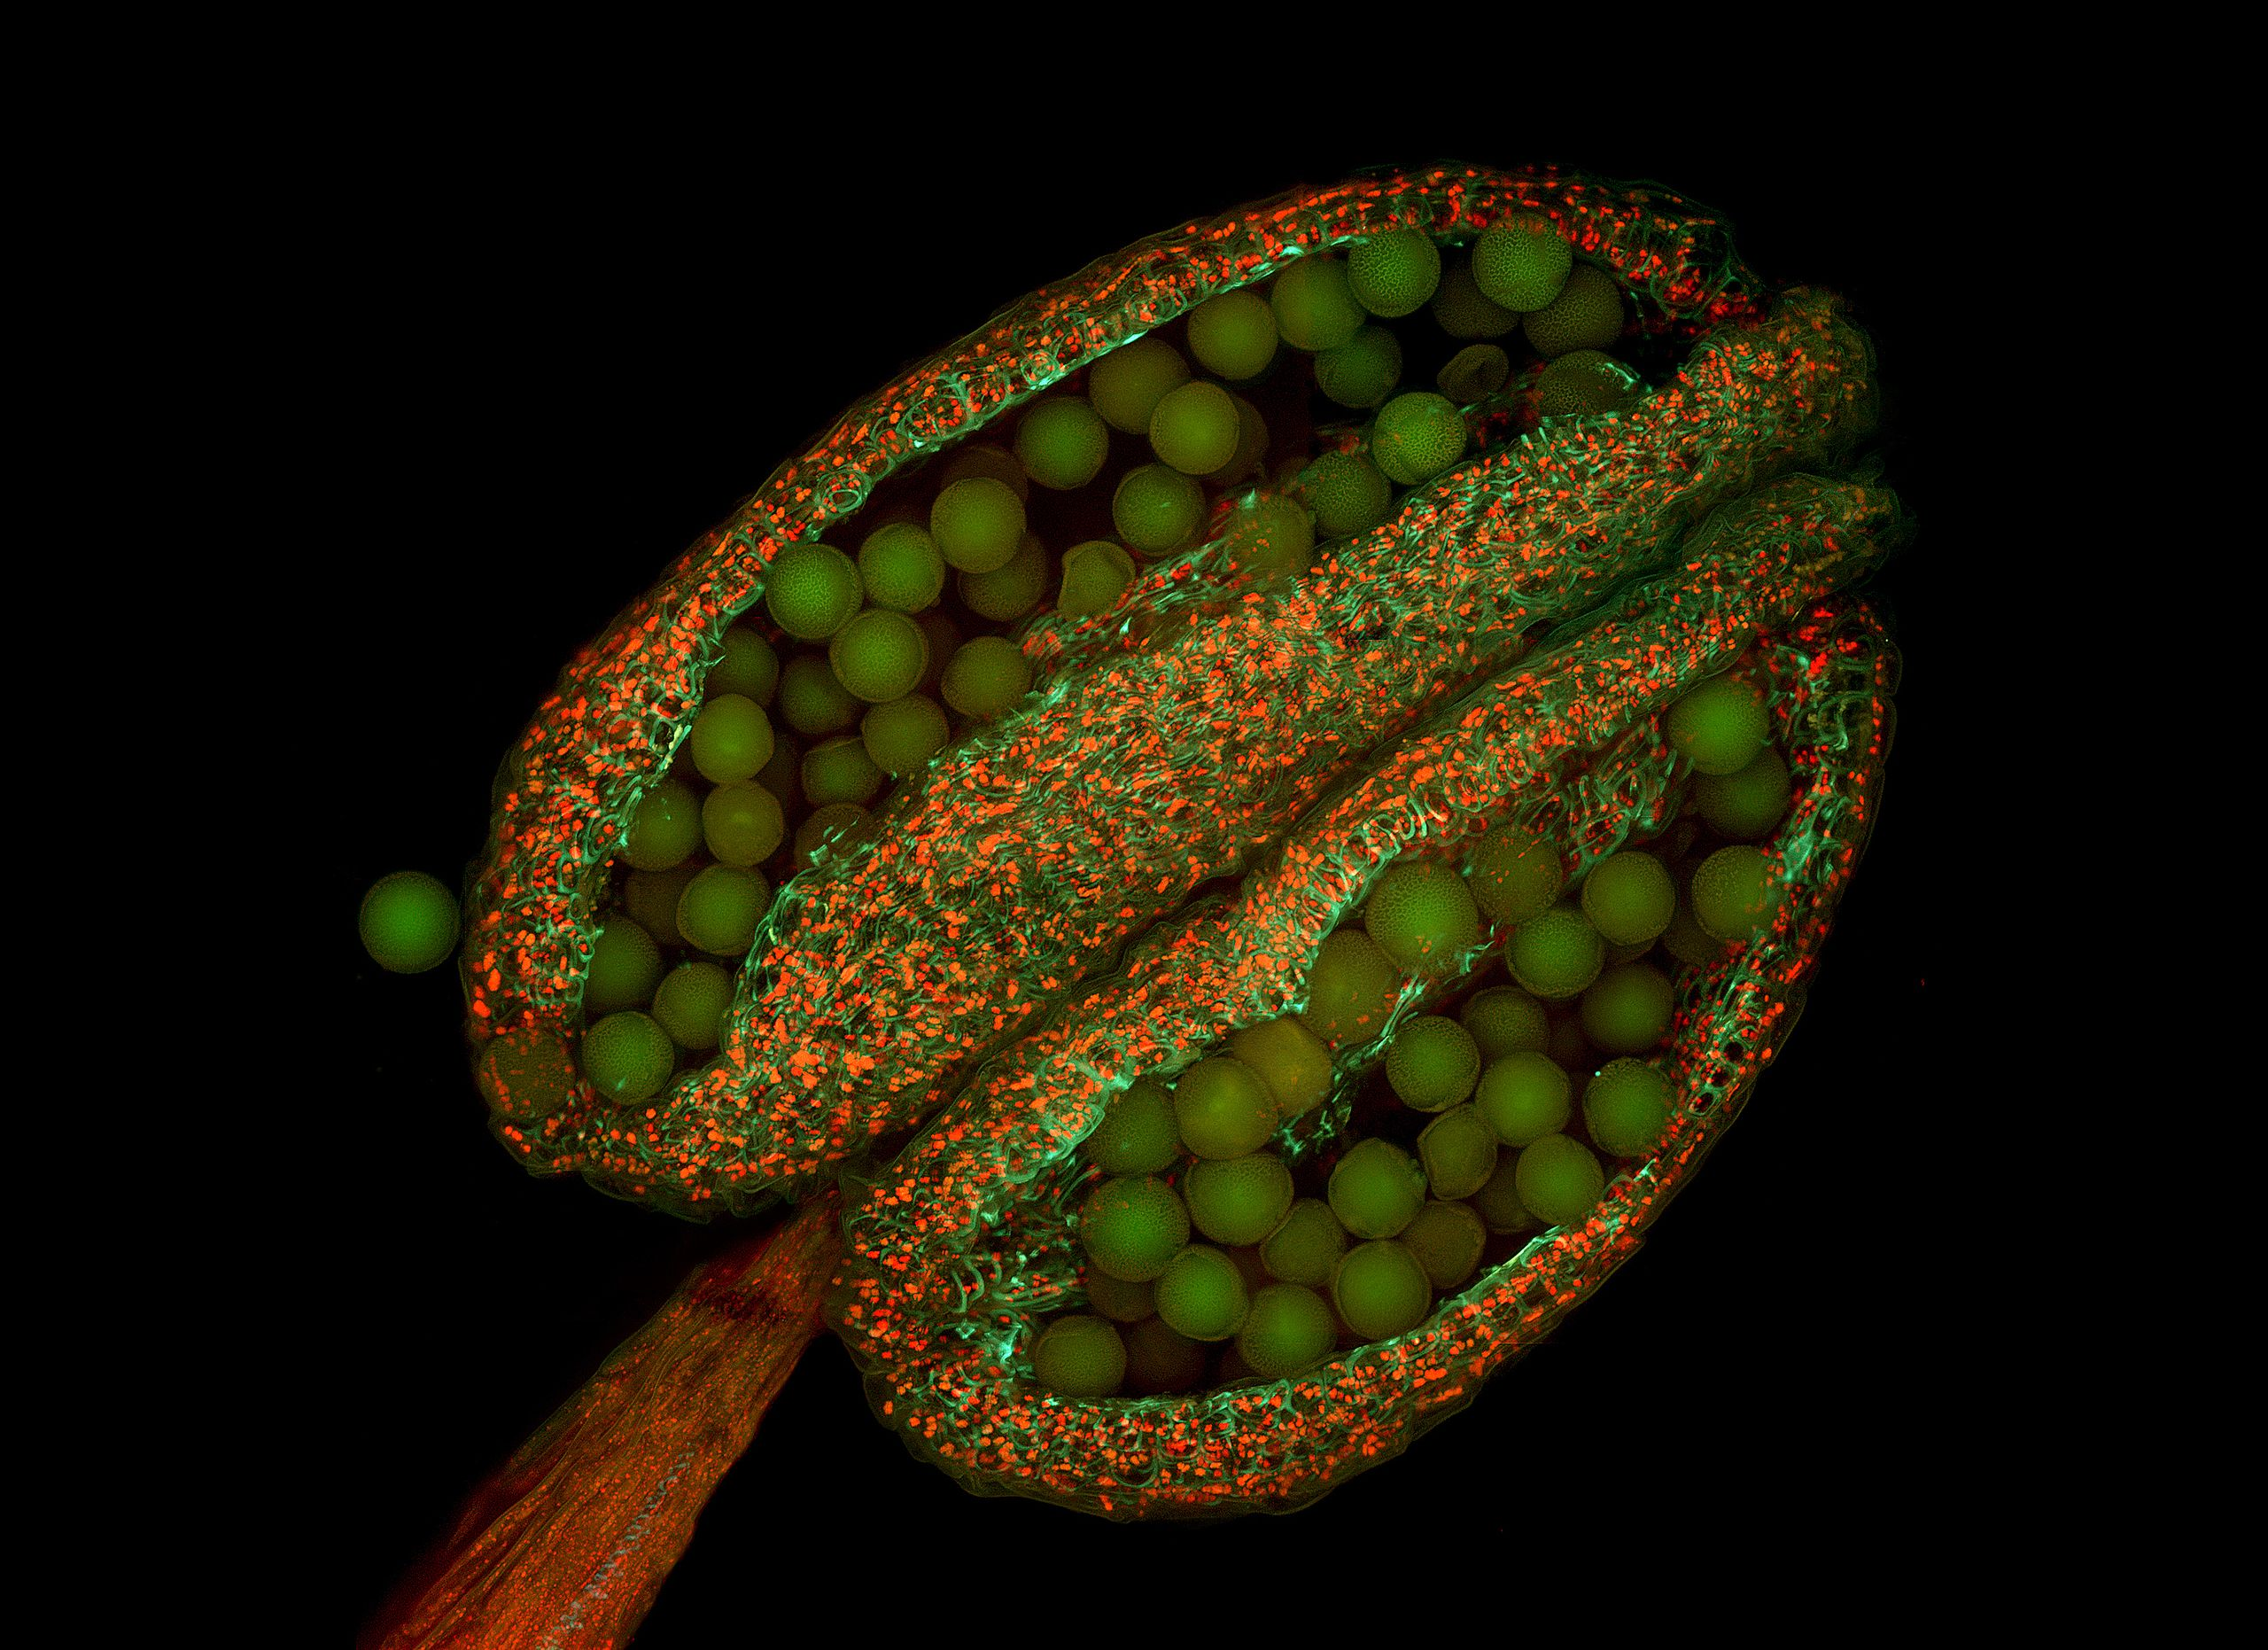
\includegraphics[width=\linewidth]{Tolmukapea.jpg}
	\caption{Anther of thale cress (Arabidopsis thaliana), fluorescence micrograph. Source: Heiti Paves, \href{https://commons.wikimedia.org/wiki/File:Tolmukapea.jpg}{https://commons.wiki-\\media.org/wiki/File:Tolmukapea.jpg}.}
	\label{fig:tcanther}
\end{figure}

Referencing a figure using its label: Figure \ref{fig:tcanther}.

Aenean porttitor eros non pharetra congue. Proin in odio in dolor luctus auctor ac et mi. Etiam euismod mi sed lectus fringilla pretium. Phasellus tristique maximus lectus et sodales. Mauris feugiat ligula quis semper luctus. Nam sit amet felis sed leo fermentum aliquet. Mauris arcu dui, posuere id sem eget, cursus pulvinar mi. Donec nec lacus non lectus fermentum scelerisque et at nibh. Sed tristique, metus ac vestibulum porta, tortor lectus placerat lorem, et convallis tellus dolor eget ante. Pellentesque dui ligula, hendrerit a purus et, volutpat tempor lectus. Mauris nec purus nec mauris rhoncus pellentesque. Quisque quis diam sed est lacinia congue. Donec magna est, hendrerit sed metus vel, accumsan rutrum nibh.

\begin{figure*} % Two column figure (notice the starred environment)
	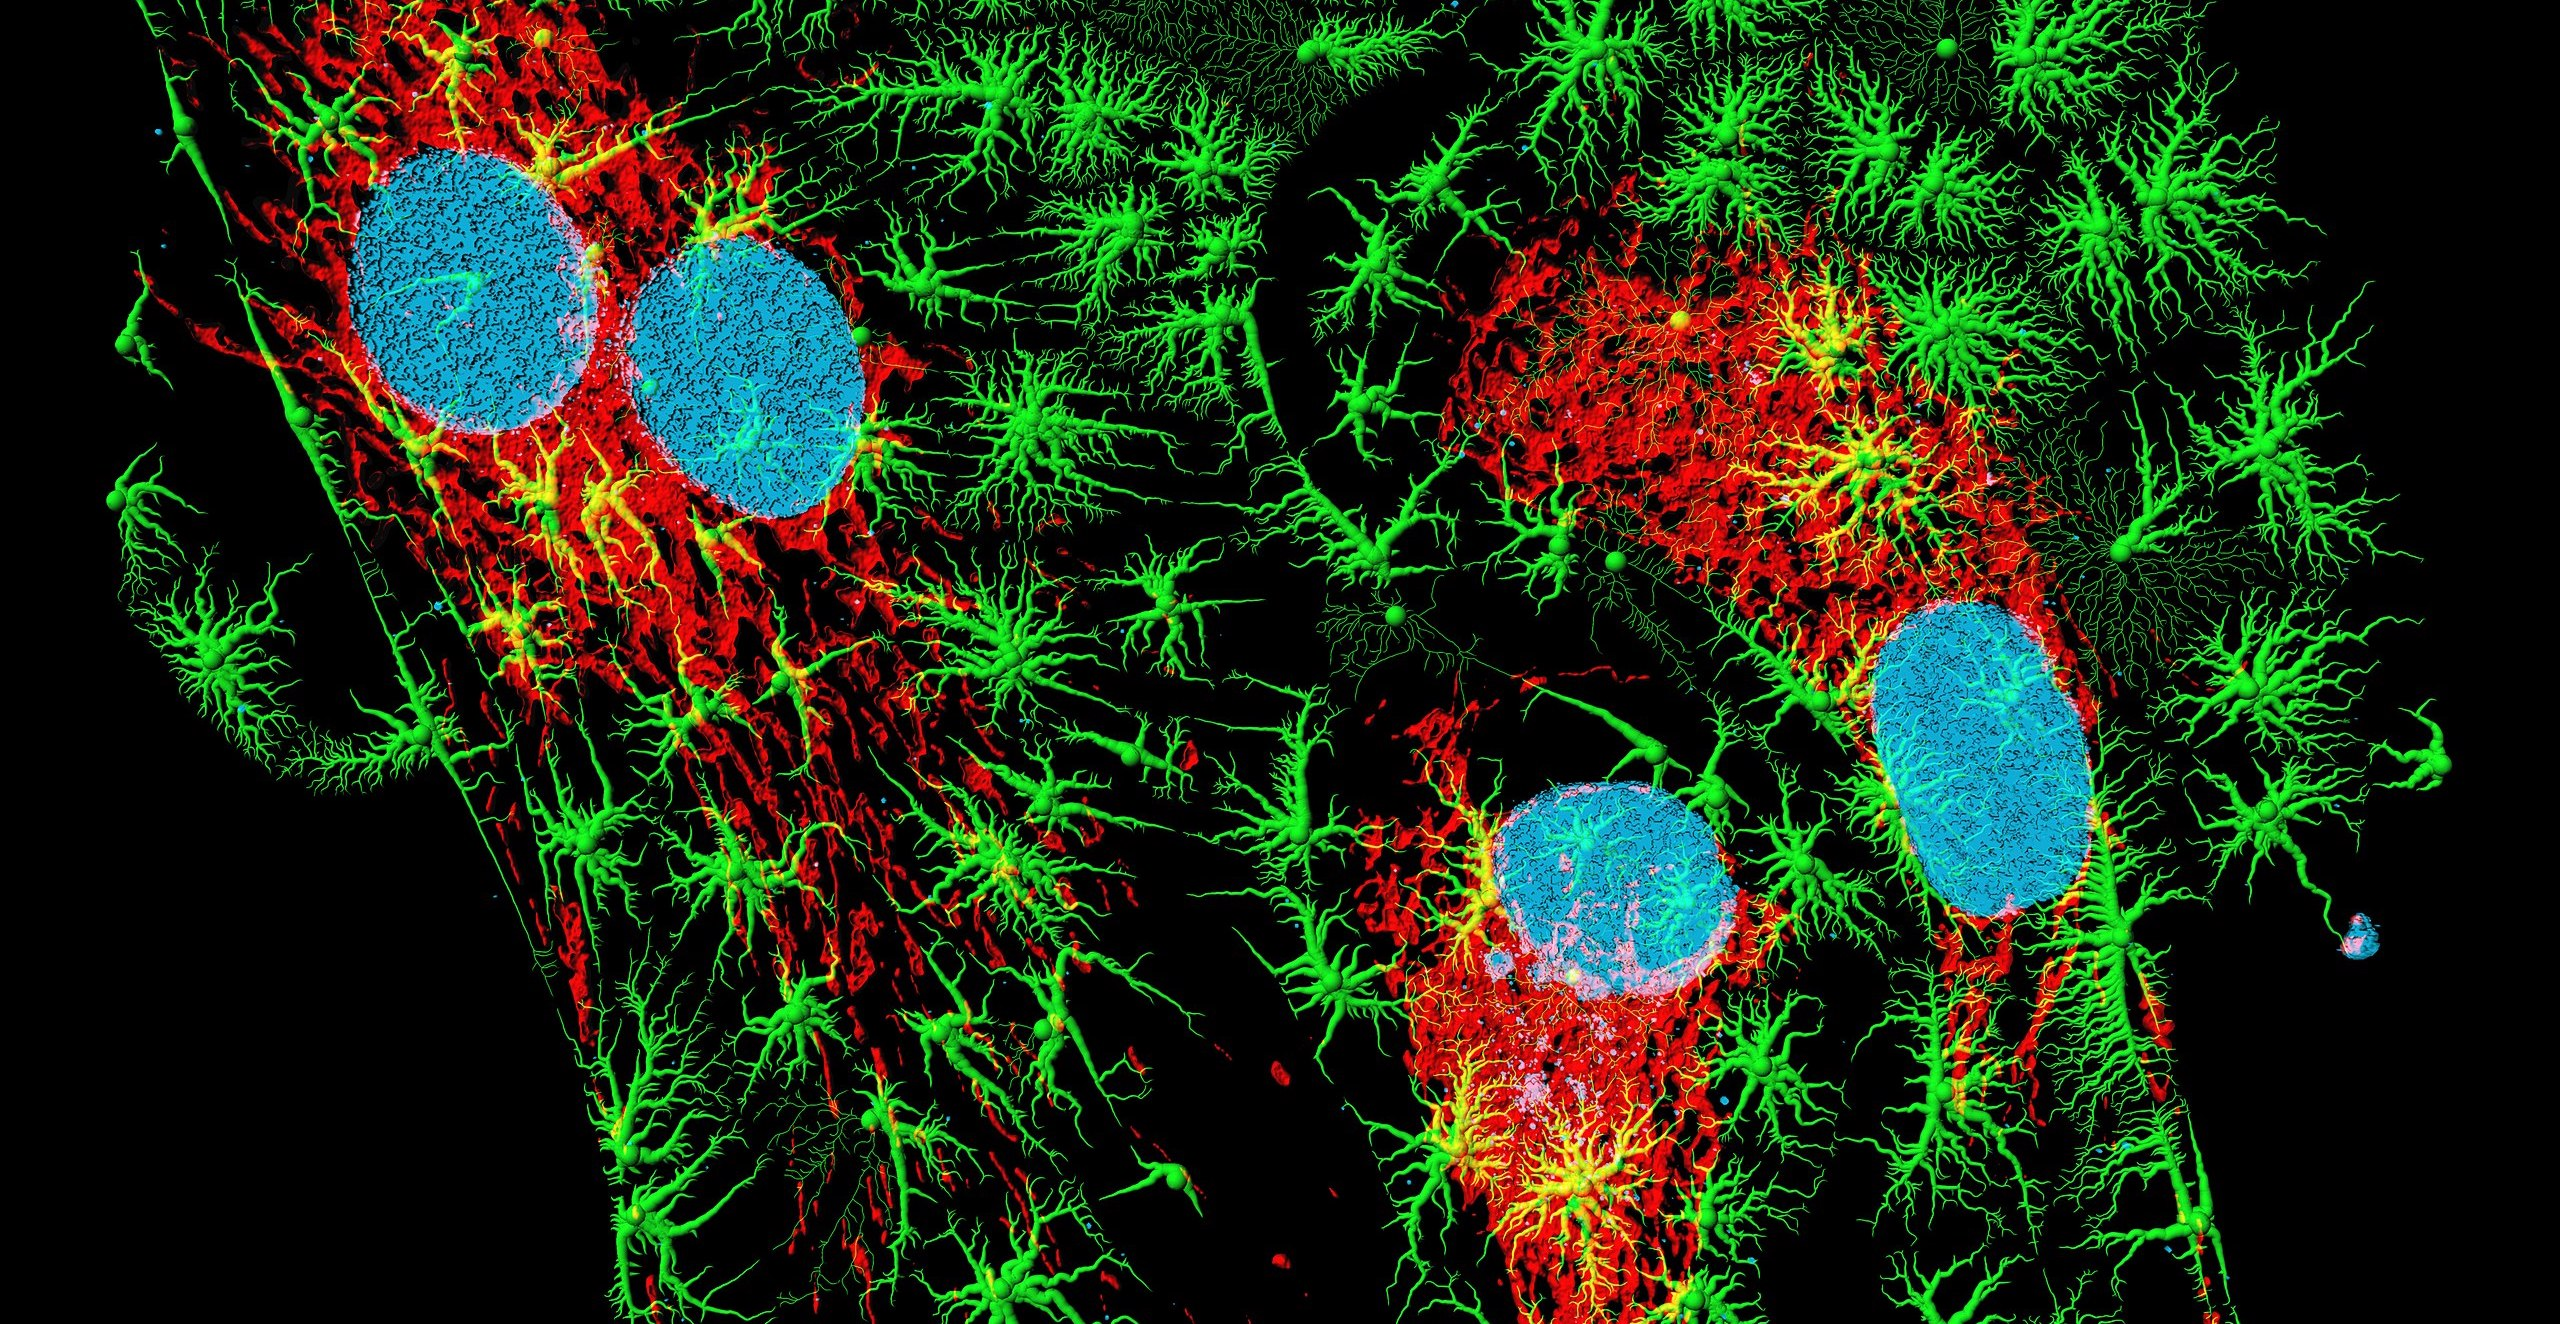
\includegraphics[width=\linewidth]{Fibroblastid.jpg}
	\caption{Bovine pulmonary artery endothelial cells in culture. Blue: nuclei; red: mitochondria; green: microfilaments. Computer generated image from a 3D model based on a confocal laser scanning microscopy using fluorescent marker dyes. Source: Heiti Paves, \href{https://commons.wikimedia.org/wiki/File:Fibroblastid.jpg}{https://commons.wikimedia.org/wiki/File:Fibroblastid.jpg}.}
	\label{fig:bpartery}
\end{figure*}

Orci varius natoque penatibus et magnis dis parturient montes, nascetur ridiculus mus. Etiam cursus lectus purus, tempus iaculis quam dictum tristique. Nam interdum sapien nec tempor mattis. Quisque id sapien nisi. Mauris vehicula ornare eros vel efficitur. Nulla consectetur, turpis quis fringilla tincidunt, mi neque iaculis lectus, vel commodo elit odio non ex. Duis facilisis, purus ac viverra iaculis, turpis lectus ultrices ante, ac vestibulum ligula magna in libero. Etiam tristique maximus lacinia. Vestibulum hendrerit, lacus malesuada laoreet blandit, sapien velit sollicitudin nunc, eu porttitor urna ligula at lorem. Aliquam faucibus eros in fermentum venenatis. Fusce consectetur congue pellentesque. Suspendisse at nisi sit amet est porttitor cursus. Cras placerat faucibus nunc, a laoreet justo dignissim sit amet.

\subsection{International Support}

\noindent àáâäãåèéêëìíîïòóôöõøùúûüÿýñçčšž

\noindent ÀÁÂÄÃÅÈÉÊËÌÍÎÏÒÓÔÖÕØÙÚÛÜŸÝÑ

\noindent ßÇŒÆČŠŽ

\subsection{Links}

This is a clickable URL link: \href{https://www.latextemplates.com}{LaTeX Templates}. This is a clickable email link: \href{mailto:vel@latextemplates.com}{vel@latextemplates.com}. This is a clickable monospaced URL link: \url{https://www.LaTeXTemplates.com}.

%------------------------------------------------

\section{Discussion}

% This statement requires citation \autocite{Smith:2023qr}. This statement requires multiple citations \autocite{Smith:2023qr, Smith:2024jd}. This statement contains an in-text citation, for directly referring to a citation like so: \textcite{Smith:2024jd}.

\subsection{Subsection One}

% Suspendisse potenti. Vivamus suscipit dapibus metus. Proin auctor iaculis ex, id fermentum lectus dapibus tristique. Nullam maximus eros eget leo pretium dapibus. Nunc in auctor erat, id interdum risus. Suspendisse aliquet vehicula accumsan. In vestibulum efficitur dictum. Sed ultrices, libero nec fringilla feugiat, elit massa auctor ligula, vehicula tempor ligula felis in lectus. Suspendisse sem dui, pharetra ut sodales eu, suscipit sit amet felis. Donec pretium viverra ante, ac pulvinar eros. Suspendisse gravida consectetur urna. Pellentesque vitae leo porta, imperdiet eros eget, posuere sem. Praesent eget leo efficitur odio bibendum condimentum sit amet vel ex. Nunc maximus quam orci, quis pulvinar nibh eleifend ac. Quisque consequat lacus magna, eu posuere tellus iaculis ac. Sed vitae tortor tincidunt ante sagittis iaculis.

\subsection{Subsection Two}

% Nullam mollis tellus lorem, sed congue ipsum euismod a. Donec pulvinar neque sed ligula ornare sodales. Nulla sagittis vel lectus nec laoreet. Nulla volutpat malesuada turpis at ultricies. Ut luctus velit odio, sagittis volutpat erat aliquet vel. Donec ac neque eget neque volutpat mollis. Vestibulum viverra ligula et sapien bibendum, vel vulputate ex euismod. Curabitur nec velit velit. Aliquam vulputate lorem elit, id tempus nisl finibus sit amet. Curabitur ex turpis, consequat at lectus id, imperdiet molestie augue. Curabitur eu eros molestie purus commodo hendrerit. Quisque auctor ipsum nec mauris malesuada, non fringilla nibh viverra. Quisque gravida, metus quis semper pulvinar, dolor nisl suscipit leo, vestibulum volutpat ante justo ultrices diam. Sed id facilisis turpis, et aliquet eros.

\subsubsection{Subsubsection Example}

% Duis venenatis eget lectus a aliquet. Integer vulputate ante suscipit felis feugiat rutrum. Aliquam eget dolor eu augue elementum ornare. Nulla fringilla interdum volutpat. Sed tincidunt, neque quis imperdiet hendrerit, turpis sapien ornare justo, ac blandit felis sem quis diam. Proin luctus urna sit amet felis tincidunt, sed congue nunc pellentesque. Ut faucibus a magna faucibus finibus. Etiam id mi euismod, auctor nisi eget, pretium metus. Proin tincidunt interdum mi non interdum. Donec semper luctus dolor at elementum. Aenean eu congue tortor, sed hendrerit magna. Quisque a dolor ante. Mauris semper id urna id gravida. Vestibulum mi tortor, finibus eu felis in, vehicula aliquam mi.

% Aliquam arcu turpis, ultrices sed luctus ac, vehicula id metus. Morbi eu feugiat velit, et tempus augue. Proin ac mattis tortor. Donec tincidunt, ante rhoncus luctus semper, arcu lorem lobortis justo, nec convallis ante quam quis lectus. Aenean tincidunt sodales massa, et hendrerit tellus mattis ac. Sed non pretium nibh. 

% Donec cursus maximus luctus. Vivamus lobortis eros et massa porta porttitor. Nam vitae suscipit mi. Pellentesque ex tellus, iaculis vel libero at, cursus pretium sapien. Curabitur accumsan velit sit amet nulla lobortis, ut pretium ex aliquam. Proin eget volutpat orci. Morbi eu aliquet turpis. Vivamus molestie urna quis tempor tristique. Proin hendrerit sem nec tempor sollicitudin.

%----------------------------------------------------------------------------------------
%	 REFERENCES
%----------------------------------------------------------------------------------------
\bibliography{daftar-pustaka}
\bibliographystyle{myapalike}
%----------------------------------------------------------------------------------------

\end{document}
